\subsection{Testing}
Si implementano i test principali per il corretto funzionamento in locale delle funzionalità del server.\\
Tutti i test condividono una funzione per simulare il database:
\begin{figure}[h!]
    \begin{center}
        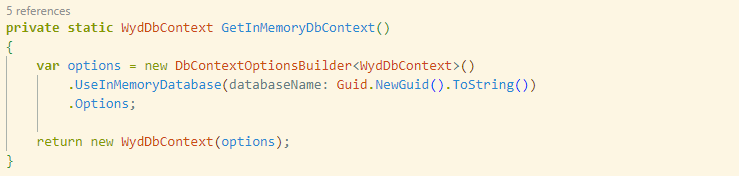
\includegraphics[width=\textwidth]{TestInit.png}
    \end{center}
\end{figure}
\subsubsection{AccountService}
\begin{figure}[h!]
    \begin{center}
        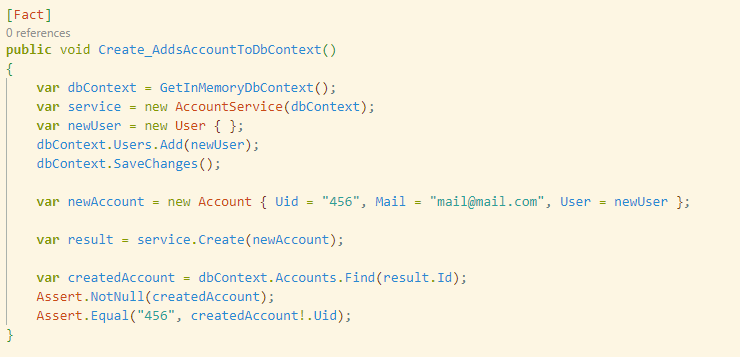
\includegraphics[width=\textwidth]{TestAccount1.png}
    \end{center}
\end{figure}
\begin{figure}[h!]
    \begin{center}
        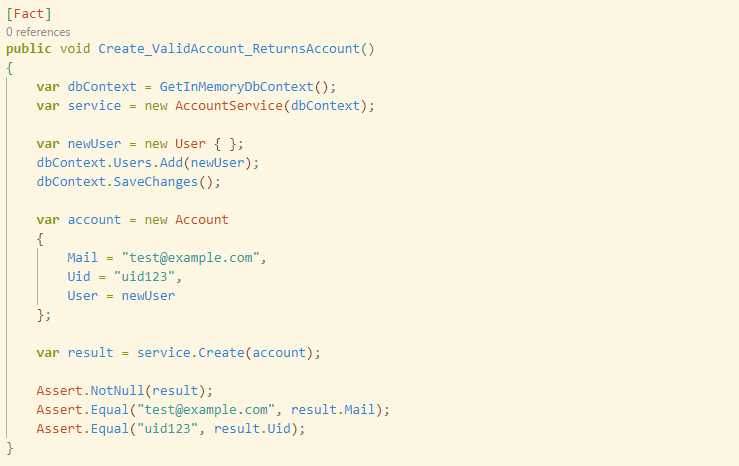
\includegraphics[width=\textwidth]{TestAccount2.png}
    \end{center}
\end{figure}
\begin{figure}[h!]
    \begin{center}
        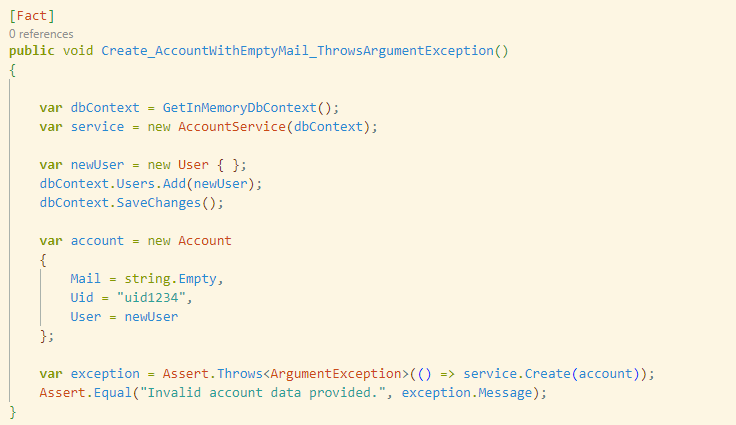
\includegraphics[width=\textwidth]{TestAccount3.png}
    \end{center}
\end{figure}
\begin{figure}[h!]
    \begin{center}
        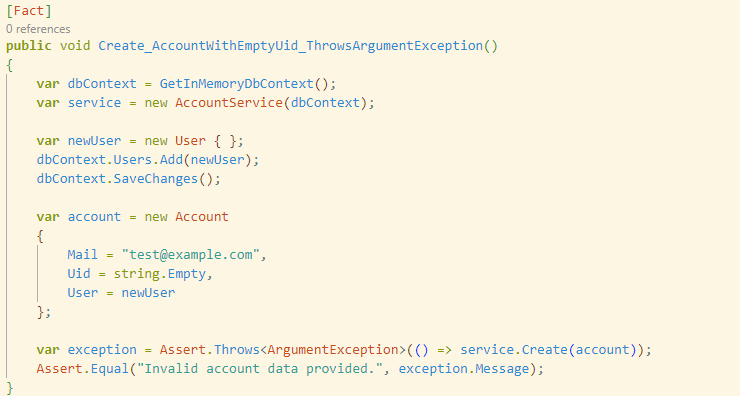
\includegraphics[width=\textwidth]{TestAccount4.png}
    \end{center}
\end{figure}
\begin{figure}[h!]
    \begin{center}
        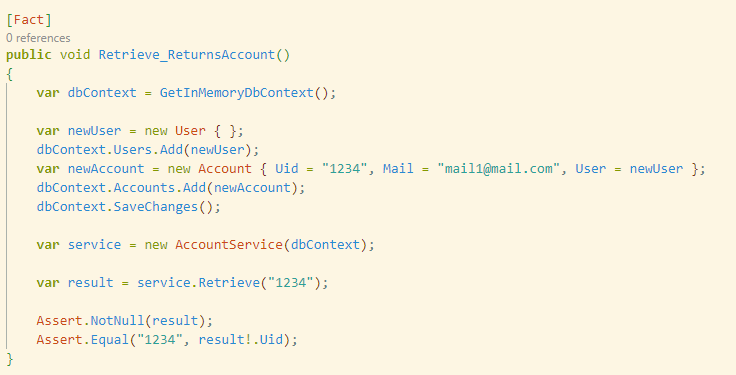
\includegraphics[width=\textwidth]{TestAccount5.png}
    \end{center}
\end{figure}
\clearpage

\subsubsection{ProfileService}
\begin{figure}[h!]
    \begin{center}
        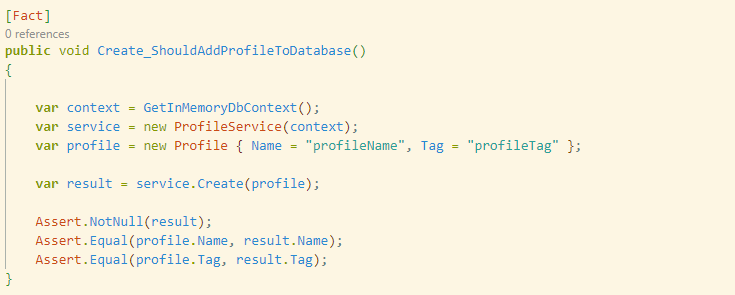
\includegraphics[width=\textwidth]{TestProfile1.png}
    \end{center}
\end{figure}
\begin{figure}[h!]
    \begin{center}
        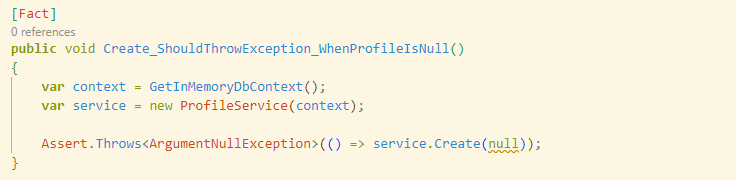
\includegraphics[width=\textwidth]{TestProfile2.png}
    \end{center}
\end{figure}
\begin{figure}[h!]
    \begin{center}
        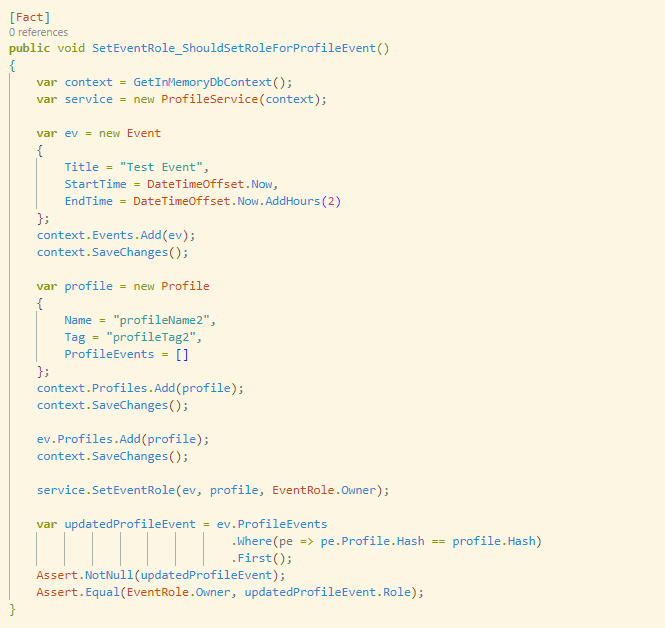
\includegraphics[width=\textwidth]{TestProfile3.png}
    \end{center}
\end{figure}
\begin{figure}[h!]
    \begin{center}
        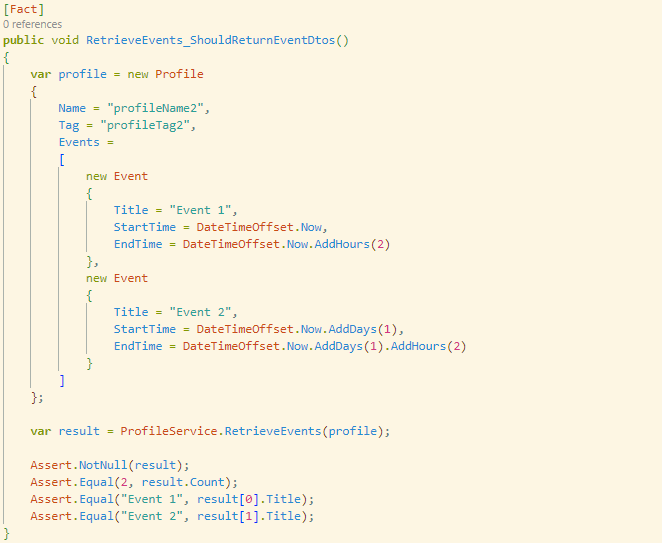
\includegraphics[width=\textwidth]{TestProfile4.png}
    \end{center}
\end{figure}
\begin{figure}[h!]
    \begin{center}
        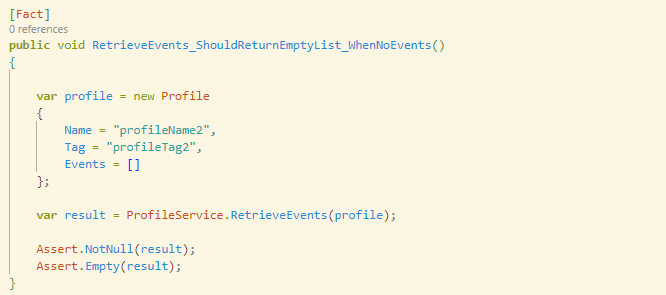
\includegraphics[width=\textwidth]{TestProfile5.png}
    \end{center}
\end{figure}
\clearpage


\subsubsection{UserService}
\begin{figure}[h!]
    \begin{center}
        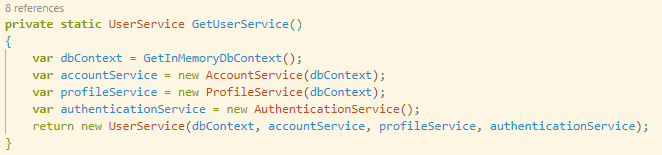
\includegraphics[width=\textwidth]{TestUserInit.png}
    \end{center}
\end{figure}
\begin{figure}[h!]
    \begin{center}
        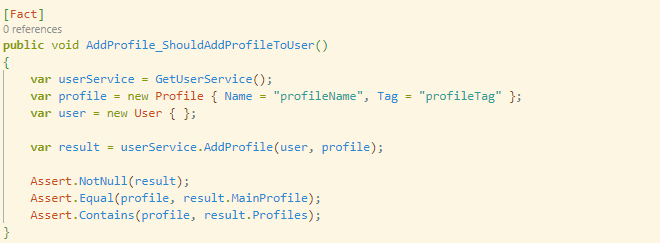
\includegraphics[width=\textwidth]{TestUser1.png}
    \end{center}
\end{figure}
\begin{figure}[h!]
    \begin{center}
        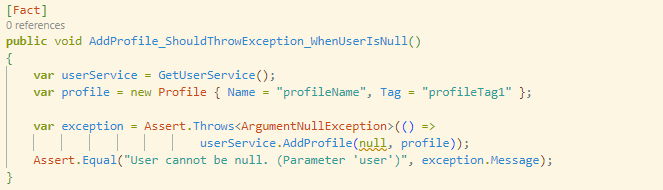
\includegraphics[width=\textwidth]{TestUser2.png}
    \end{center}
\end{figure}
\begin{figure}[h!]
    \begin{center}
        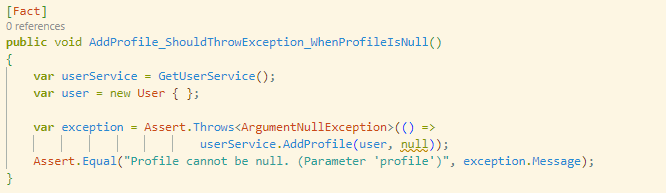
\includegraphics[width=\textwidth]{TestUser3.png}
    \end{center}
\end{figure}
\begin{figure}[h!]
    \begin{center}
        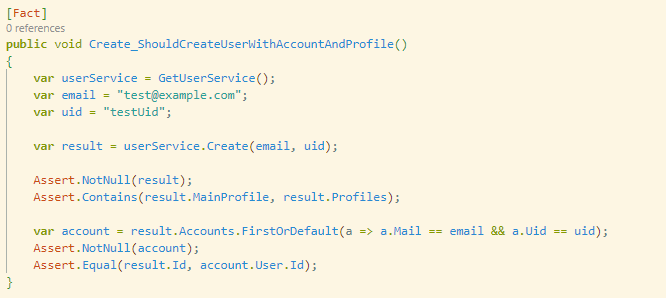
\includegraphics[width=\textwidth]{TestUser4.png}
    \end{center}
\end{figure}
\begin{figure}[h!]
    \begin{center}
        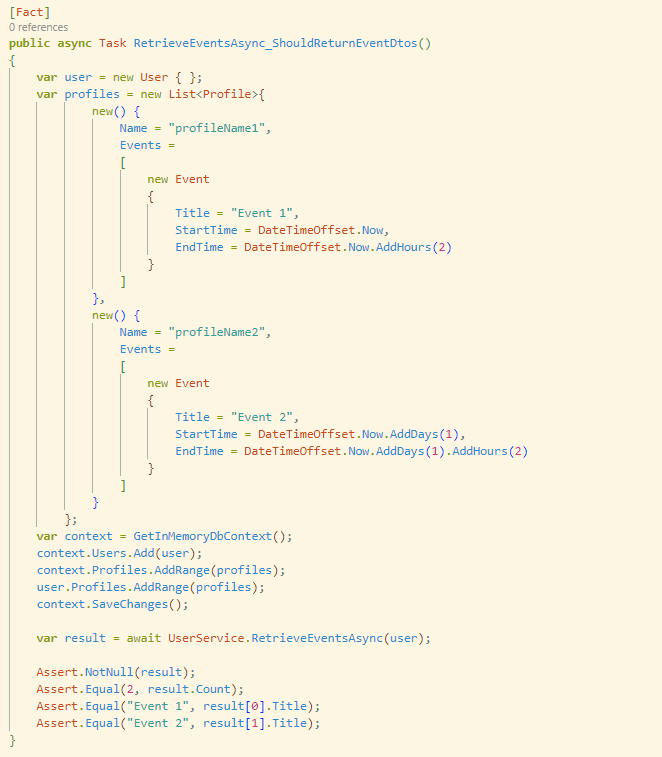
\includegraphics[width=\textwidth]{TestUser5.png}
    \end{center}
\end{figure}
\begin{figure}[h!]
    \begin{center}
        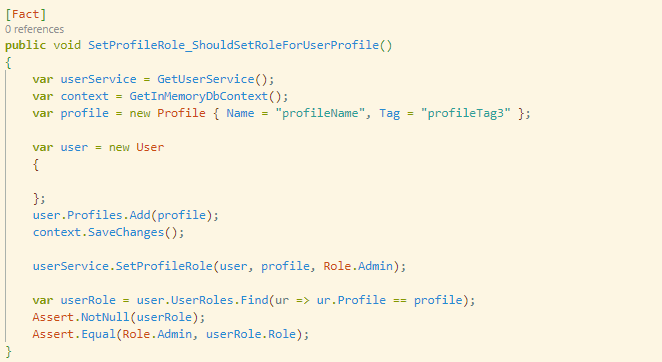
\includegraphics[width=\textwidth]{TestUser6.png}
    \end{center}
\end{figure}
\begin{figure}[h!]
    \begin{center}
        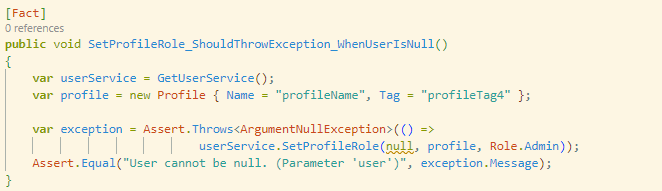
\includegraphics[width=\textwidth]{TestUser7.png}
    \end{center}
\end{figure}
\begin{figure}[h!]
    \begin{center}
        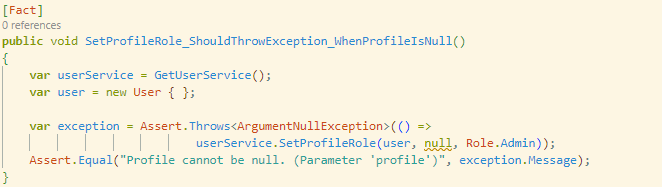
\includegraphics[width=\textwidth]{TestUser8.png}
    \end{center}
\end{figure}
\begin{figure}[h!]
    \begin{center}
        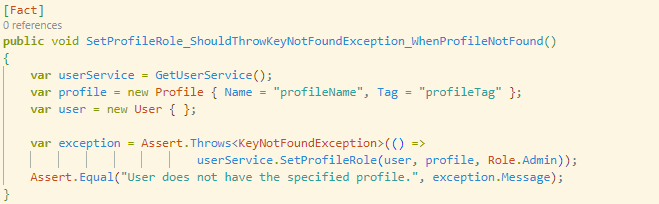
\includegraphics[width=\textwidth]{TestUser9.png}
    \end{center}
\end{figure}
\clearpage

\subsubsection{EventService}
\begin{figure}[h!]
    \begin{center}
        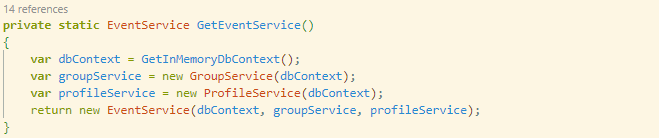
\includegraphics[width=\textwidth]{TestEventInit.png}
    \end{center}
\end{figure}
\begin{figure}[h!]
    \begin{center}
        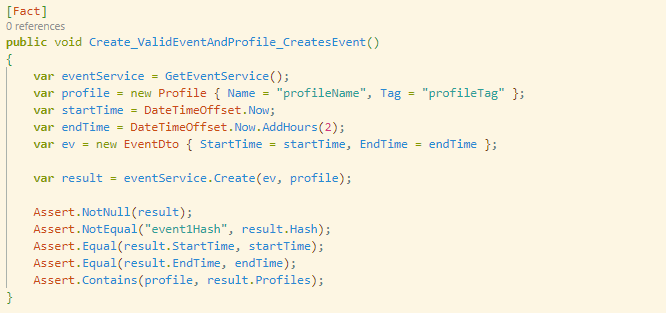
\includegraphics[width=\textwidth]{TestEvent1.png}
    \end{center}
\end{figure}
\begin{figure}[h!]
    \begin{center}
        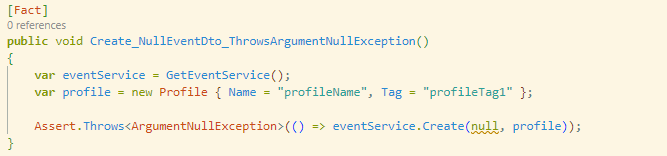
\includegraphics[width=\textwidth]{TestEvent2.png}
    \end{center}
\end{figure}
\begin{figure}[h!]
    \begin{center}
        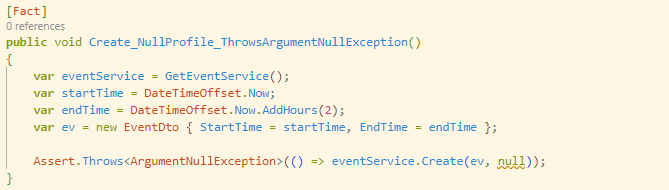
\includegraphics[width=\textwidth]{TestEvent3.png}
    \end{center}
\end{figure}
\begin{figure}[h!]
    \begin{center}
        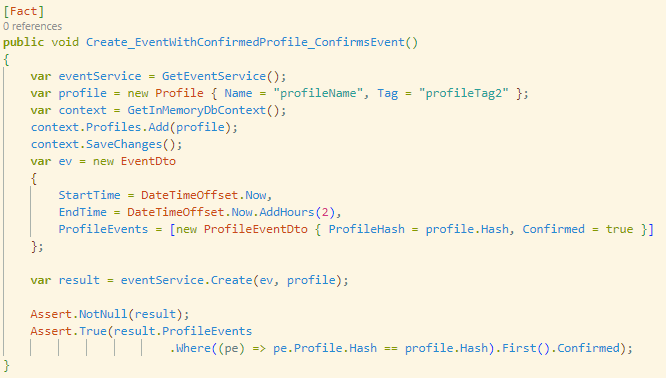
\includegraphics[width=\textwidth]{TestEvent4.png}
    \end{center}
\end{figure}
\begin{figure}[h!]
    \begin{center}
        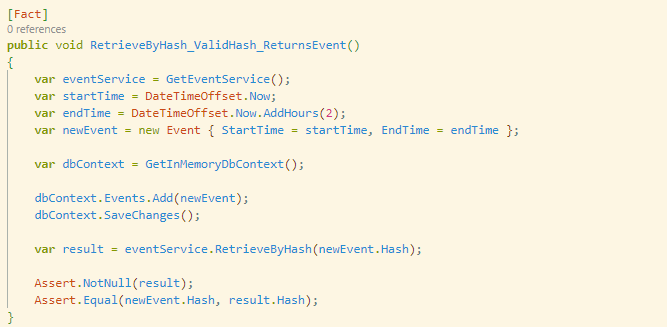
\includegraphics[width=\textwidth]{TestEvent5.png}
    \end{center}
\end{figure}
\begin{figure}[h!]
    \begin{center}
        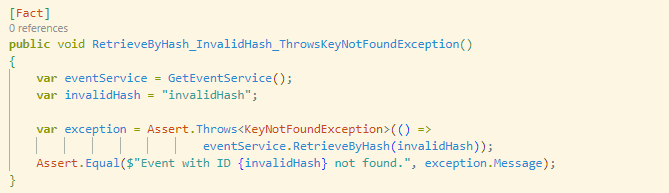
\includegraphics[width=\textwidth]{TestEvent6.png}
    \end{center}
\end{figure}
\begin{figure}[h!]
    \begin{center}
        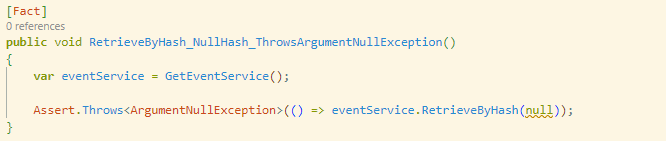
\includegraphics[width=\textwidth]{TestEvent7.png}
    \end{center}
\end{figure}
\begin{figure}[h!]
    \begin{center}
        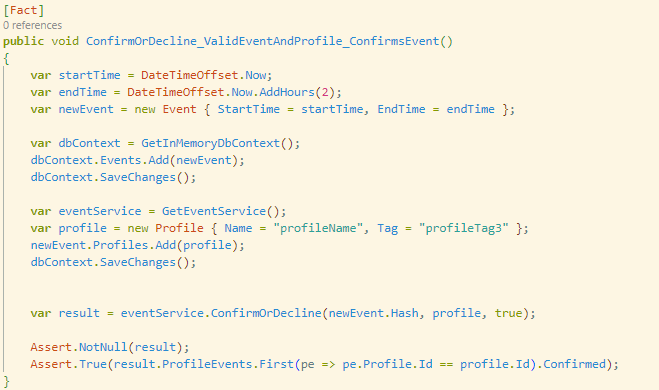
\includegraphics[width=\textwidth]{TestEvent8.png}
    \end{center}
\end{figure}
\begin{figure}[h!]
    \begin{center}
        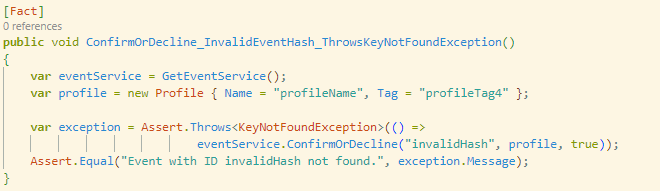
\includegraphics[width=\textwidth]{TestEvent9.png}
    \end{center}
\end{figure}\begin{figure}[h!]
    \begin{center}
        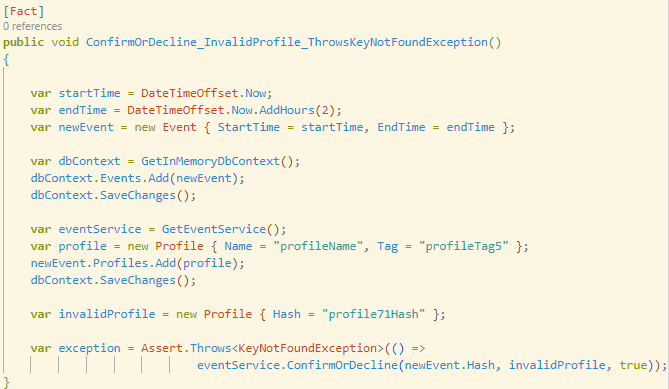
\includegraphics[width=\textwidth]{TestEvent10.png}
    \end{center}
\end{figure}
\begin{figure}[h!]
    \begin{center}
        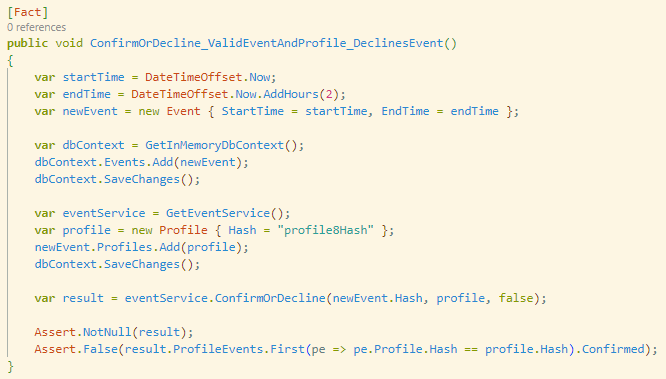
\includegraphics[width=\textwidth]{TestEvent12.png}
    \end{center}
\end{figure}
\begin{figure}[h!]
    \begin{center}
        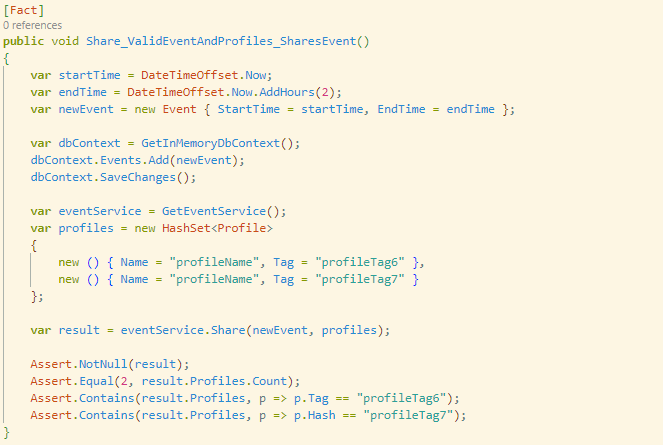
\includegraphics[width=\textwidth]{TestEvent13.png}
    \end{center}
\end{figure}
\begin{figure}[h!]
    \begin{center}
        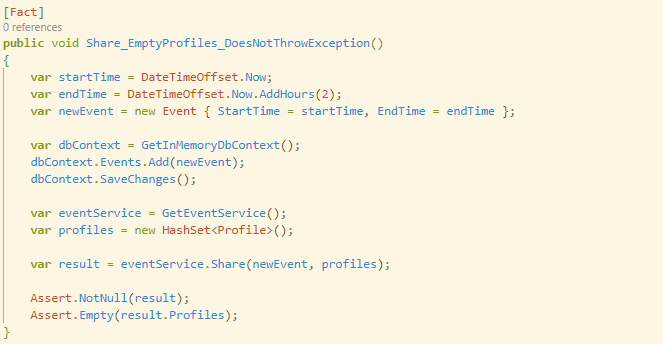
\includegraphics[width=\textwidth]{TestEvent14.png}
    \end{center}
\end{figure}
\begin{figure}[h!]
    \begin{center}
        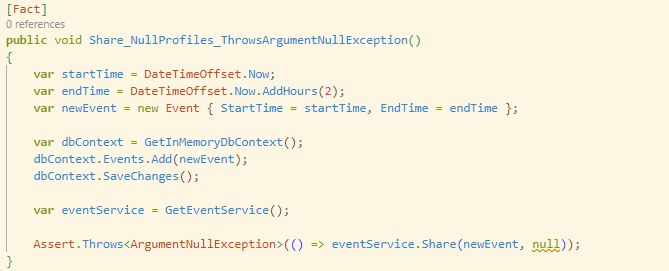
\includegraphics[width=\textwidth]{TestEvent15.png}
    \end{center}
\end{figure}

\clearpage